\chapter{Exercises with answers}

\begin{Exercise} [
  title={Chromosomes},
  difficulty={1},
  label={ex1},
  origin={G. Valle}
 ]

  In adult human cells there are 46 chromosomes. De novo mutations are generally
very rare and we are not considering them in the following reasoning.
Answer \textbf{True} or \textbf{False}:

  \Question 23 chromosome are inherited from the mother and 23 from the father
  \Question Each chromosome of a child must have an identical copy in one of the
2 parents
  \subQuestion Explain why
\end{Exercise}

\begin{Answer} [
   ref={ex1},
   number={1}
 ]

  \Question True
  \Question False
  \subQuestion The second statement is wrong because of the crossing over

\end{Answer}


\begin{Exercise} [
  title={Genomes and genes},
  difficulty={1},
  label={ex2},
  origin={G. Valle}
 ]

  Approximately, how big is the genome and how many genes are there...

  \Question In a bacterium like \textbf{E. Coli}
  \Question In a simple eukaryote like \textbf{yeast}
  \Question In humans

\end{Exercise}

\begin{Answer} [
  ref={ex2},
  number={2}
 ]

  \Question Genome size: 100 Mbp. Number of genes: 19000 (27\% encoding)
  \Question Genome size: 13 Mbp. Number of genes: 6000 (70\% encoding)
  \Question Genome size: 3000 Mbp. Number of genes: 23000/25000 (1.5\% encoding)

\end{Answer}

\begin{Exercise} [
  title={Enzyme},
  difficulty={1},
  label={ex3},
  origin={G. Valle}
 ]

  Answer the questions.

  \Question How is called the enzyme that duplicate the DNA?
  \Question How is called the enzyme that transcribes DNS into RNA?
  \Question How is it called the biological structure where proteins are
synthesized?
\end{Exercise}

\begin{Answer} [
  ref={ex3},
  number={3}
 ]

  \Question DNA Polymerase
  \Question RNA Polymerase
  \Question Ribosome
\end{Answer}

\begin{Exercise} [
  title={DeBruijn assembly},
  difficulty={2},
  label={exA},
  origin={G. Valle}
 ]

We want to discover the sequence of a hypothetical very small single stranded
genome, with an estimated length of 20 bases.

For this purpose, the 19 shotgun reads listed below were produced.

Unfortunately, the sequencing technology was not very good and some sequencing
errors may be possible.

You should attempt to assemble the genome with the DeBruijn graph method,
using \textbf{kmers of 4 bases}.

Consider that there are 256 different kmers of 4 bases.

\begin{figure}[H]
  \centering
  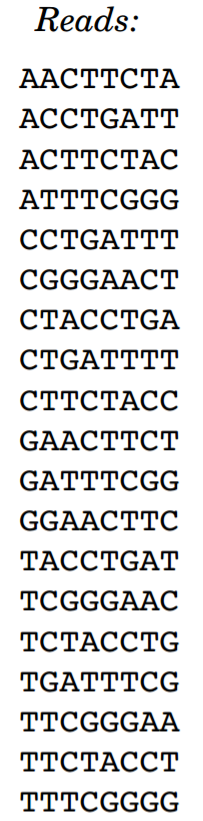
\includegraphics[scale=0.3]{reads_exA}
  \caption{Reads}
  \label{fig:reads}
\end{figure}

  \Question You should check if all the kmer occur more or less at the expected
level and you should consider possible repeated regions or kmers arising from
sequencing errors.

  \Question You should draw and analyse the resulting graph to establish if
there is one or more Eulerian cycles and if there is any evidence to establish
whether the original genome was linear or circular.

  \Question You should write the final circular genomic sequence.

Finally, you can further think about the peculiarity of this genome and why
DeBruijn graph are used, instead than full length reads.
\end{Exercise}

\begin{Answer} [
  ref={exA},
  number={6}
 ]

  \Question

\begin{tabular}{ | l | r | }
  \hline
  \textbf{Kmer} & \textbf{Count} \\ \hline
  \texttt{AACT} & 4 \\ \hline
  \texttt{ACTT} & 4 \\ \hline
  \texttt{ACCT} & 5 \\ \hline
  \texttt{ATTT} & 5 \\ \hline
  \texttt{CTTC} & 5 \\ \hline
  \texttt{CCTG} & 5 \\ \hline
  \texttt{CTGA} & 5 \\ \hline
  \texttt{CTAC} & 5 \\ \hline
  \texttt{CGGG} & 5 \\ \hline
  \texttt{TTCT} & 5 \\ \hline
  \texttt{TCTA} & 5 \\ \hline
  \texttt{TGAT} & 5 \\ \hline
  \texttt{TTTC} & 4 \\ \hline
  \texttt{TTCG} & 5 \\ \hline
  \texttt{TCGG} & 5 \\ \hline
  \texttt{TACC} & 5 \\ \hline
  \texttt{TTTT} & 1 \\ \hline
  \texttt{GATT} & 5 \\ \hline
  \texttt{GGGA} & 3 \\ \hline
  \texttt{GGAA} & 4 \\ \hline
  \texttt{GAAC} & 4 \\ \hline
  \texttt{GGGG} & 1 \\ \hline
\end{tabular}

Pheraps the reads \texttt{TTTT} and \texttt{GGGG} should be considered as
sequencing errors.

  \Question To be completed
  \Question To be completed
\end{Answer}

